\documentclass{article}

\usepackage[pctex32]{graphics}
\usepackage{amssymb}
\usepackage[left=3cm,top=2cm,right=3cm,nohead,nofoot]{geometry}
\usepackage{latexsym}
\usepackage{epsfig}
\usepackage{float}
\parindent0pt
\parskip6pt
%\pagestyle{empty}
%\usepackage{fancybox}
\usepackage{pstricks}
\newcommand{\R}{{\mathbb R}}
\title{Image Reconstruction using Tikhonov Regularization}
\author{Duttaabhinivesh Devathi}
\begin{document}
\maketitle

\bigskip
{\Large {\bf Summary}}
\bigskip

The assignment deals with reconstructing an image after blurring it using a standard Gaussian blur.

\bigskip
{\Large {\bf Looking at the Original Image}}
\bigskip

The image is in Figure~\ref{fig:Figure 1} and is represented using the command \texttt{imagesc(X)} in Matlab. It is represented as a matrix $X \in \mathbb{R}^{100\times100}$.

\begin{figure}[h!]
\centerline{
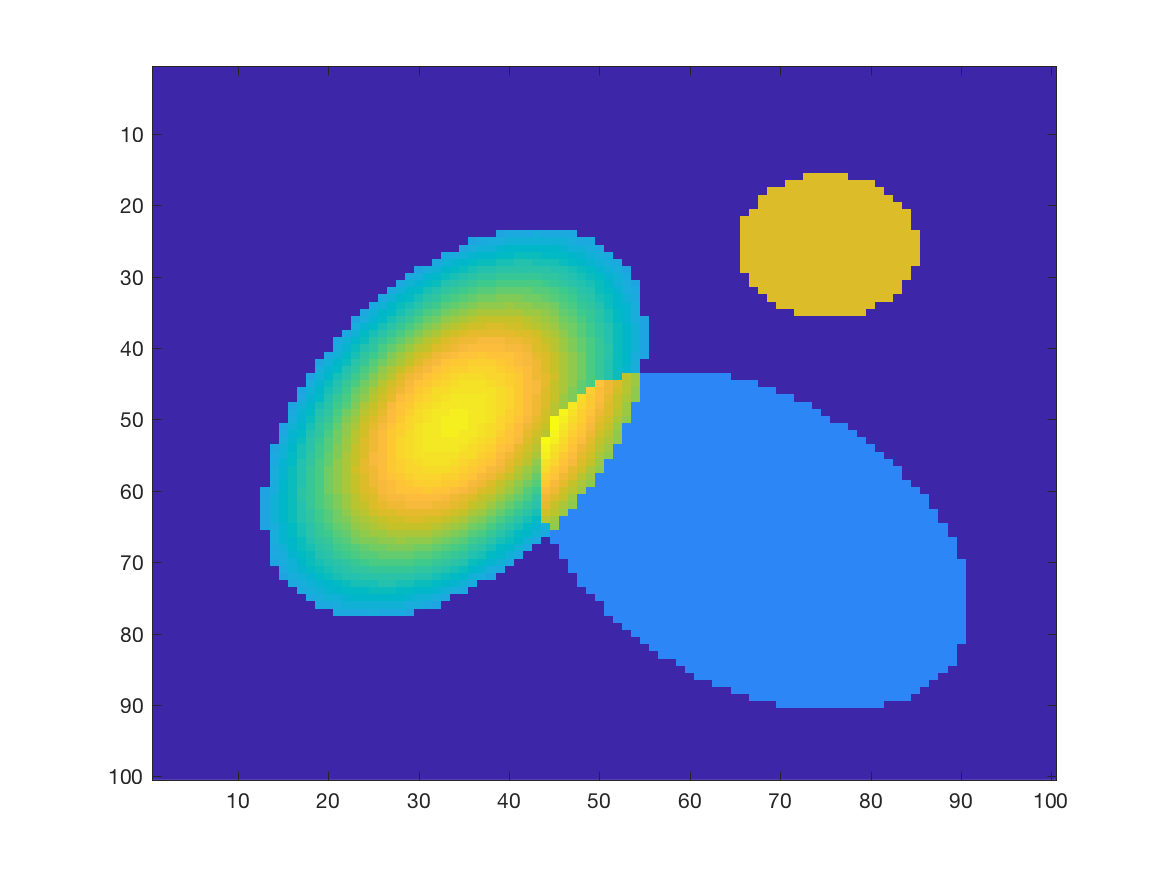
\includegraphics[width= 14cm]{TrueTarget.png}
}
\caption{\label{fig:Figure 1} Image before any processing.}
\end{figure}

\newpage
{\Large {\bf Constructing a Gaussian Blurring Kernel}}
\bigskip

Here, we create the matrix A which represents a blurring kernel of the image so that we can set up the inverse problem. 

First, we want to do these operations using a linear transformation, so we take the image and represent it in a vector form. In general, if the image is $X \in \mathbb{R}^{n_{1}\times n_{2}}$, then we want the image to be in vector form as $x \in \mathbb{R}^{n_{1}n_{2} \times 1}$ where the columns of the matrix are stacked on top of each other.

Thus, we can set up a convolution kernel $A \in \mathbb{R}^{n_{1}n_{2} \times n_{1}n_{2}}$ in block structure such that each block on the diagonal of A transforms each successive column of $X$. In this case, $X \in \mathbb{R}^{100\times 100}$, so $A \in \mathbb{R}^{10^4 \times 10^4}$.

The truncated Gaussian kernel depends on the integer lattice points of the actual indices of the values of the matrix. In a crude way, the further away two pixels are, the less of a blurring effect there will be. To set this up in Matlab, it's given with the following code. 

\begin{verbatim}
n1 = 100;
n2 = 100;
N = n1*n2; % Number of pixels
p1 = (1:n1);
p2 = (1:n2);
[P1,P2] = meshgrid(p1,p2);
P = [P2(:)’;P1(:)’]; % First row = index to the matrix row, second to column
\end{verbatim}

From the assignment, we set up the matrix such that

\[A_{jk} = \exp(-\frac{1}{2\lambda^2} ||P(:,j) - P(:,k)||^2)\].

Each column of the matrix $P$ is such that the first entry is the row of the image pixel and the second entry is the column of the image pixel. The convolution kernel blurs the image based on the distance of the pixels, so along the main diagonal the matrix is all $\mathsf 1$ and as you move away from the diagonal the value gets smaller.

One concern of this matrix is its size. Many of the values far from the main diagonal will be numerically zero, but not represented as such in its computation. For this reason, we calculate the entry only if it crosses a certain threshold. The code for this is given below.

\begin{verbatim}
lambda = 3;
syms tau 
tau = double(solve(exp(-tau^2/(2*lambda^2)) == 10^-3, tau > 0));
A = zeros(N);

for j = 1:N
    for k = 1:N
        distnc = norm(P(:,j) - P(:,k))^2;
        if (distnc < tau) % Remove all the entries that are too spread apart
            A(j,k) = exp(-distnc/(2*lambda^2));
        end
    end
end
A = sparse(A); % reducing the file size of the matrix (gets rids of zeros).
\end{verbatim}

We can visualize the sparsity structure of the matrix using the Matlab commands \texttt{imagesc(A)} and \texttt{spy(A)}.

\begin{figure}[H]
\centerline{
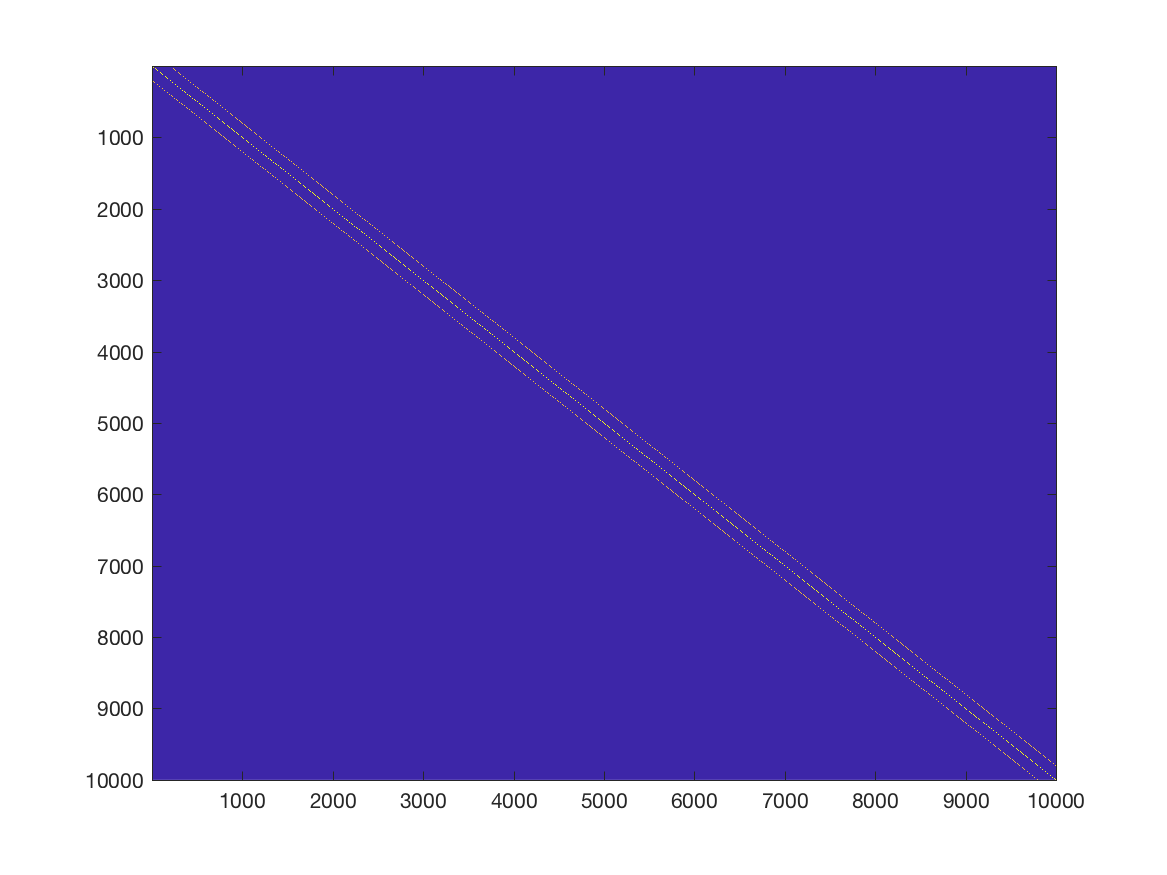
\includegraphics[width= 9cm]{imagesc(A).png} 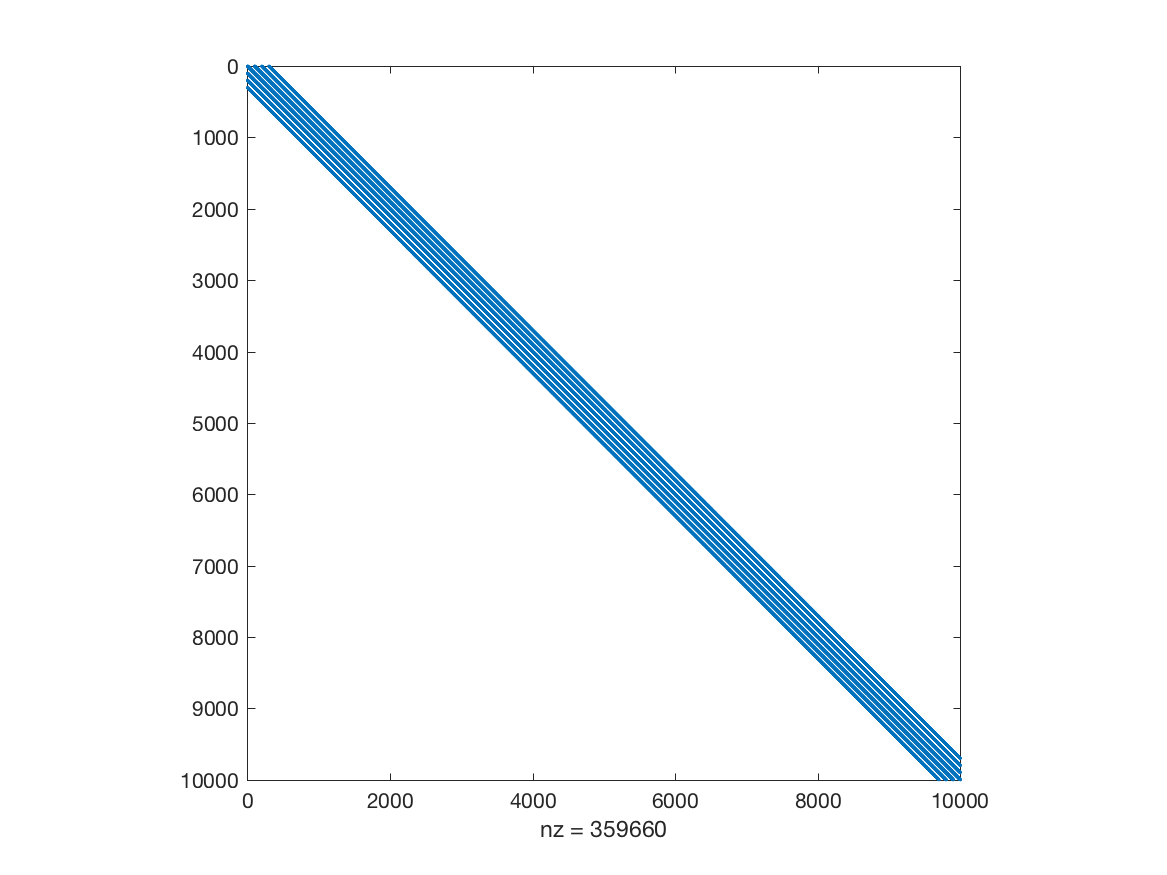
\includegraphics[width = 9cm]{spy(A).png}
}
\caption{\label{fig:Figure 2} Sparsity structure of A. Left panel uses \texttt{imagesc(A)} and right panel uses \texttt{spy(A)}.}
\end{figure}

As you can see in Figure~\ref{fig:Figure 2}, the matrix $\mathbb A$ is a diagonal matrix where the first few super diagonals are filled and the rest are 0.

\bigskip
{\Large {\bf Blurred Image}}
\bigskip

The blurred matrix is taken by applying $\mathbb A$ to the image in vector form, and reshaping:

\begin{verbatim}
imvec = X(:); % Image in Vector Format
x_blur = A*imvec;
X_blur = reshape(x_blur, [100, 100]);
imagesc(X_blur)
print('BlurredTarget','-dpng')
\end{verbatim}

\begin{figure}[H]
\centerline{
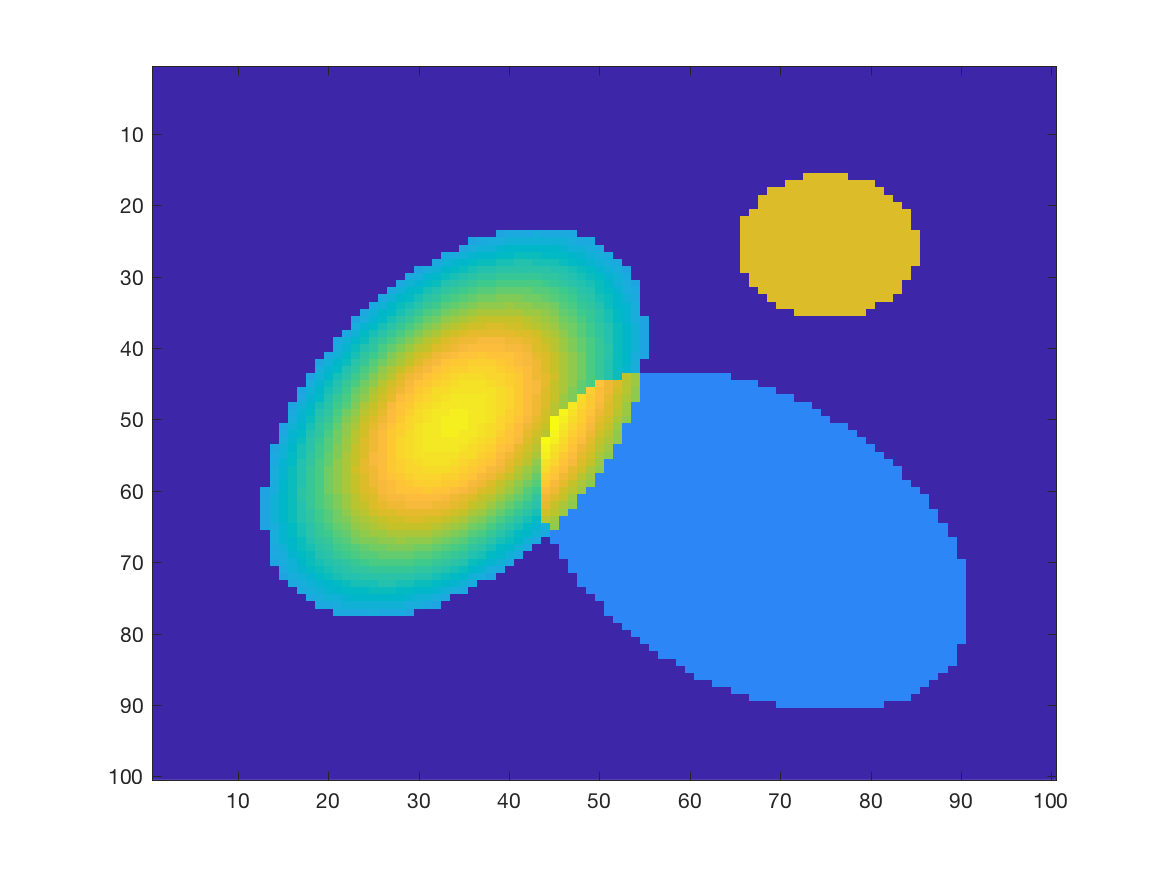
\includegraphics[width = 7cm]{TrueTarget.png} 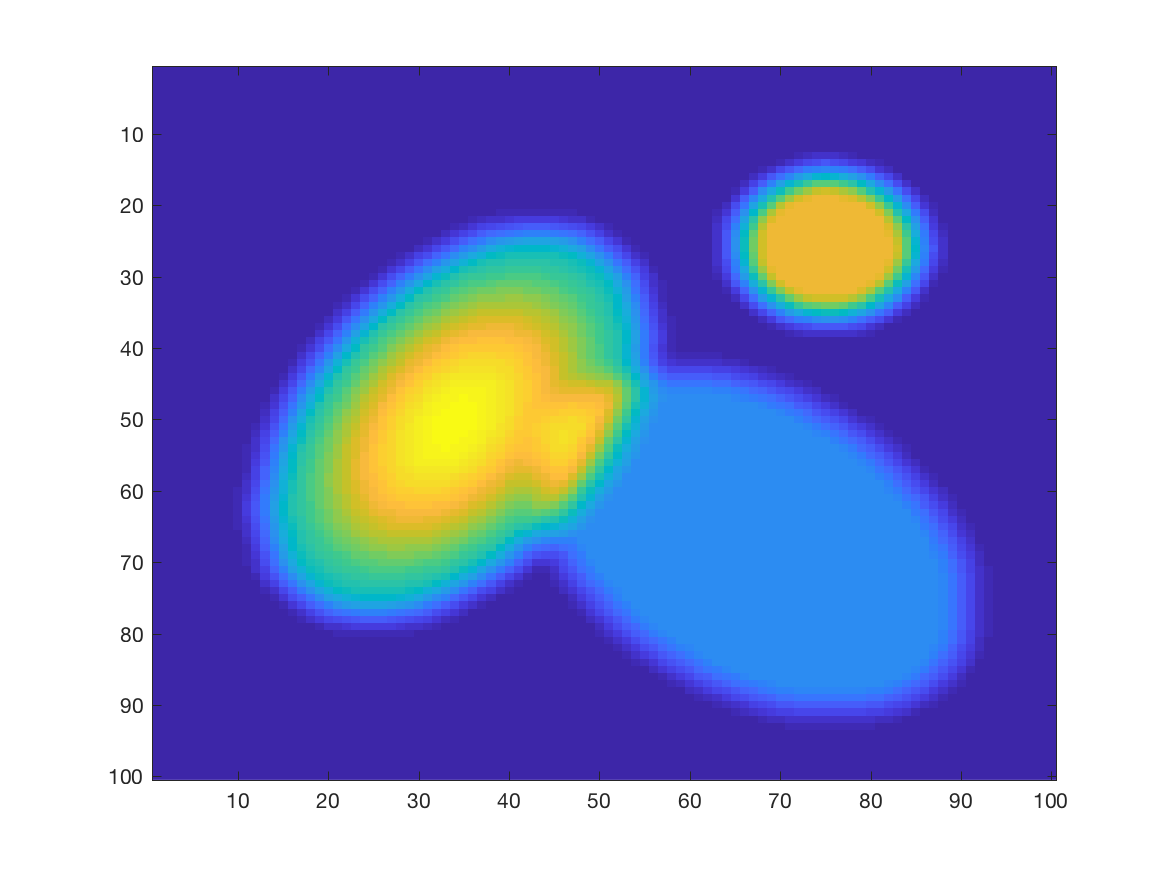
\includegraphics[width = 7cm]{blurredTarget.png}
}
\caption{\label{fig:Figure 3} The left panel shows the original image and the right panel shows the blurred image.}
\end{figure}

\bigskip
{\Large {\bf Reconstruction Using Tikhonov Regularization}}
\bigskip

Tikhonov regularization can be summarized with the following equation:

\[
\mathsf{x_{\alpha} = argmin{||b - Ax||^2 + \alpha||x||^2}}.
\]

We want to visualize the reconstruction using the Tikhonov Regularization with $\mathsf{L = I}$ as in the equation above. First, let's try visualizing this image for $\mathsf{\alpha} = 10^{-6}$.

\begin{figure}[H]
\centerline{
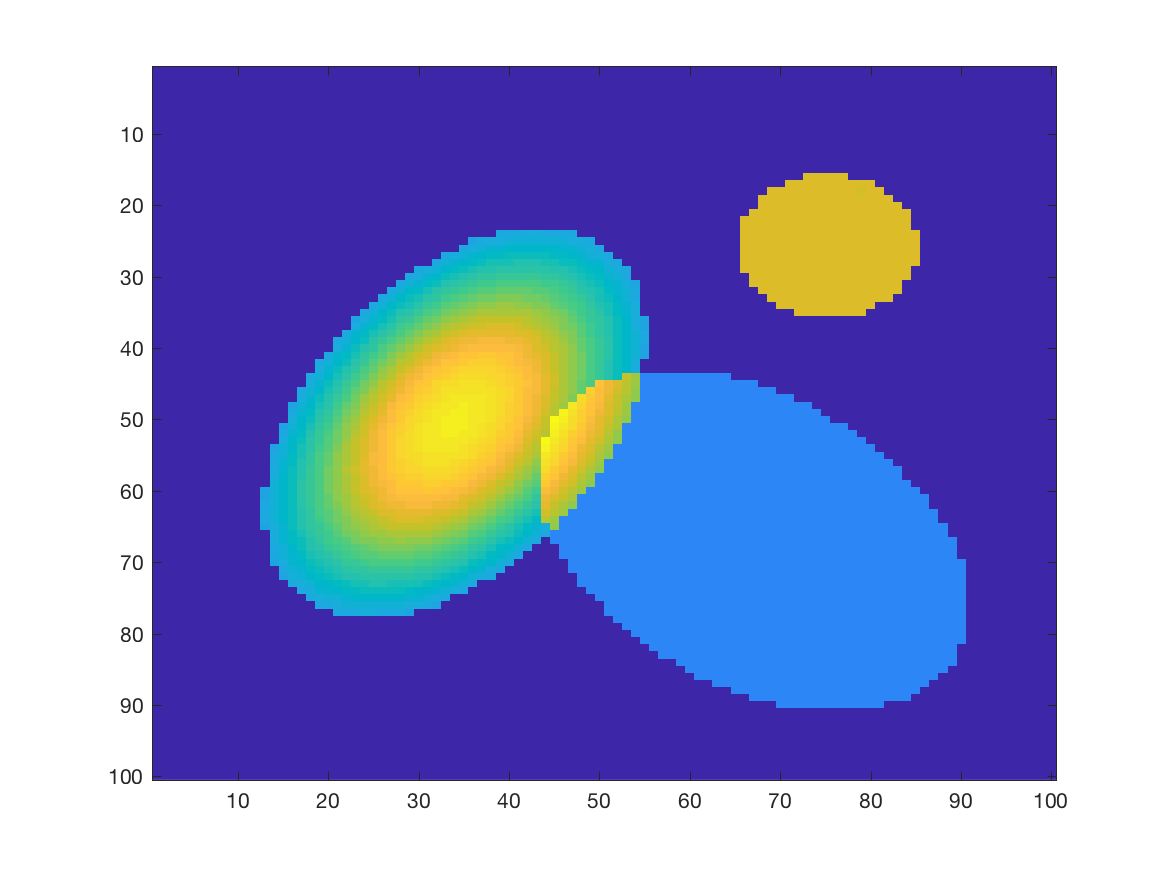
\includegraphics[width = 8cm]{alpha1e-6.png} 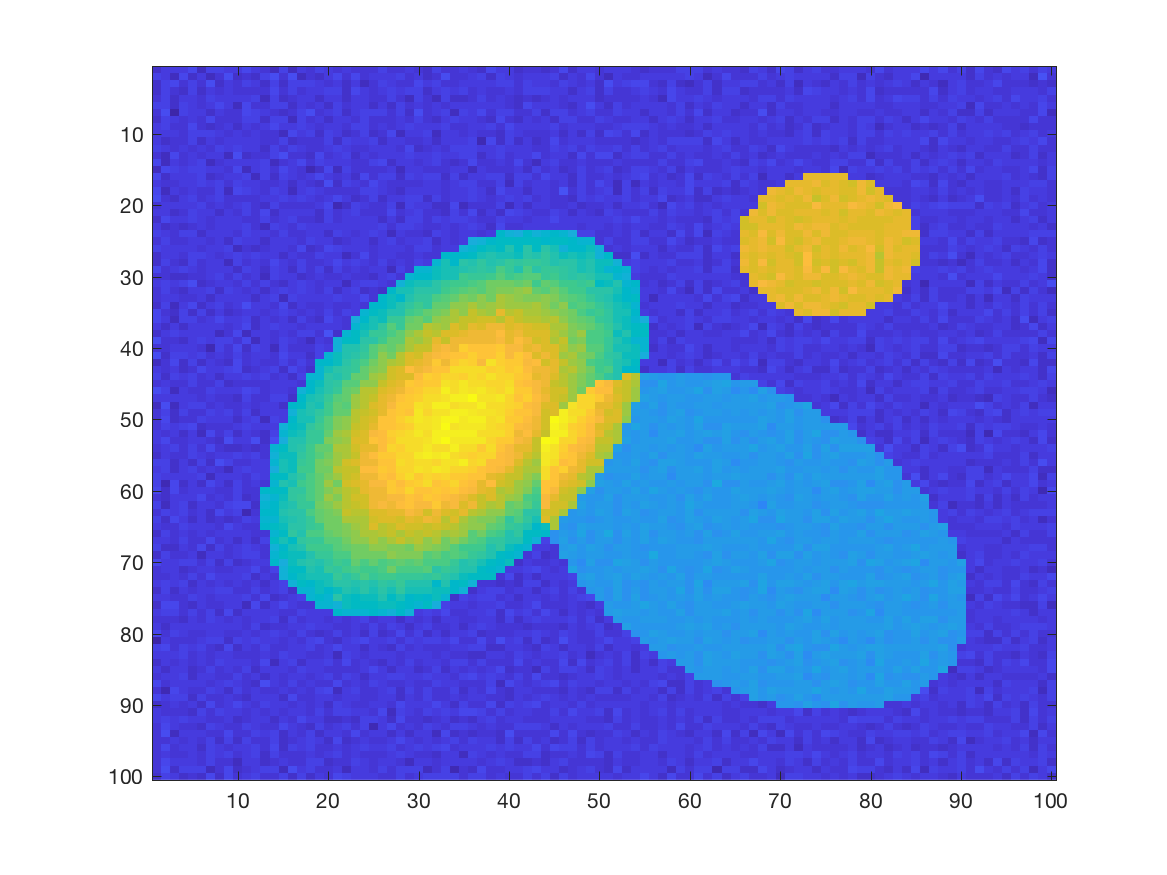
\includegraphics[width = 8cm]{alpha1e-6_noise.png}
}
\caption{\label{fig:Figure 4} Both these images are tikhinov regularized with $\mathsf{\alpha = 10^{-6}}$. The left panel shows the reconstructed image without any noise and the right panel has a reconstructed image that perturbs the image with some noise of magnitude $\mathsf{10^{-3}}$.}
\end{figure}

The images were constructed with the following code:

\begin{verbatim}
%% Tikhonov Regularization - Reconstruction for alpha = 1e-6
alpha = 1e-6;
noiselev = 1e-3;
noise = noiselev*randn(N,1);
r = [b; zeros(N,1)];

x_alpha = (A'*A + alpha*eye(N))\(A'*b); % reconstructed image L = I
discr = norm(x_blur - A*x_alpha);
imagesc(reshape(x_alpha, [100, 100]))
print('alpha1e-6', '-dpng')

bnoise = b + noise;
x_alpha = (A'*A + alpha*eye(N))\(A'*bnoise); % reconstructed image L = I
discr_noise = norm(x_blur - A*x_alpha);
imagesc(reshape(x_alpha, [100, 100]))
print('alpha1e-6_noise', '-dpng')
\end{verbatim}

Now, we find the reconstruction of the image using the Morozov Discrepancy principle. The text states that the regularization parameter is found using a geometric bisection algorithm to find the optimal $\alpha$. 

\begin{figure}[H]
\centerline{
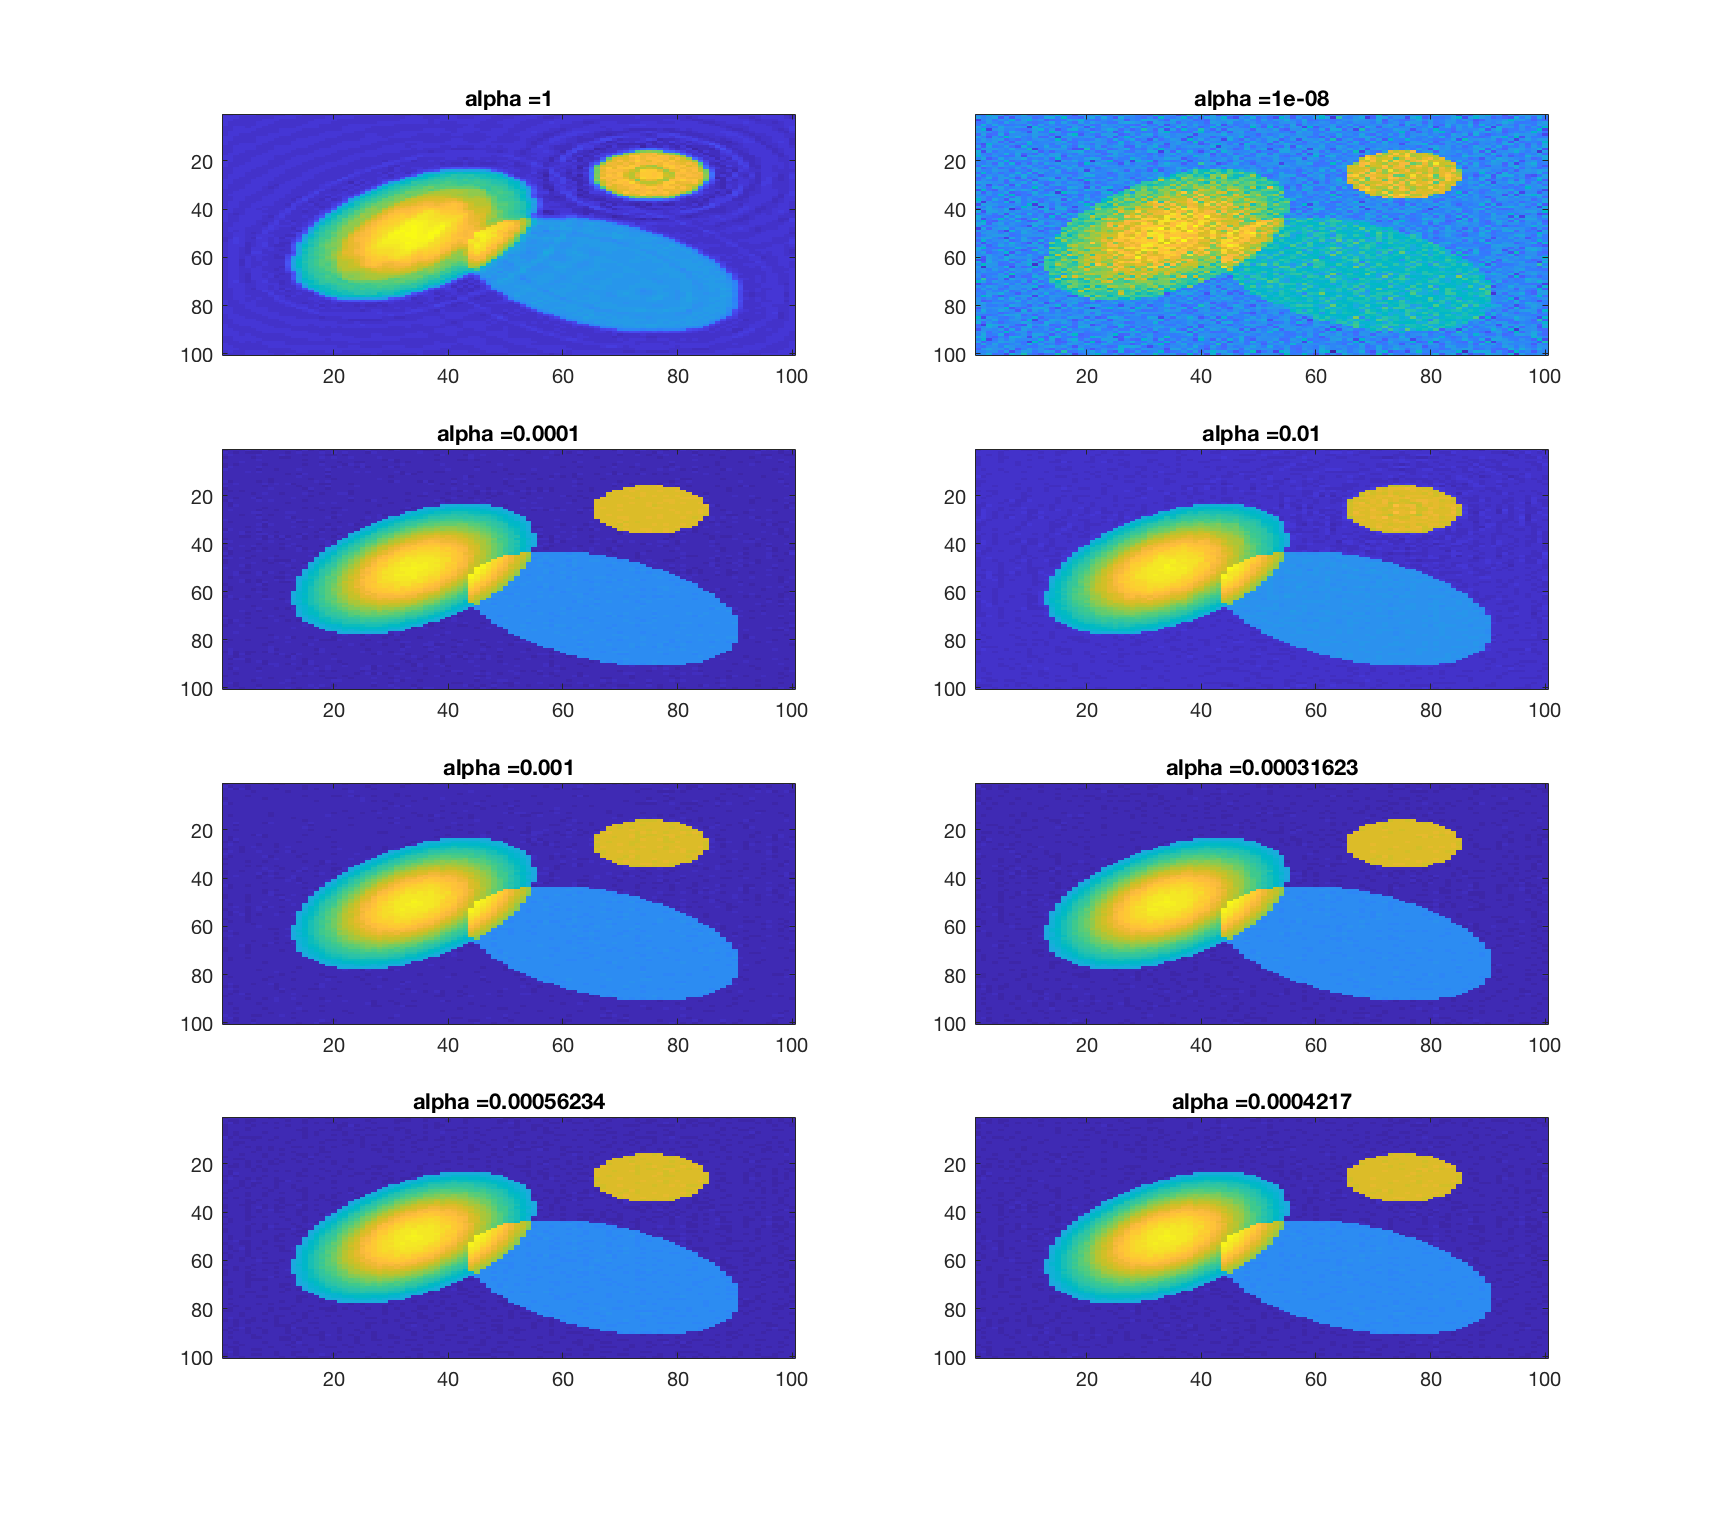
\includegraphics[width = 20cm]{evolution.png}
}
\caption{\label{fig:Figure 5} This shows the evolution of the solution by computing the solution using Tikhonov Regularization and finding the optimal regularization parameter $\alpha$ by a geometric bisection algorithm.}
\end{figure}



\begin{figure}[H]
\centerline{
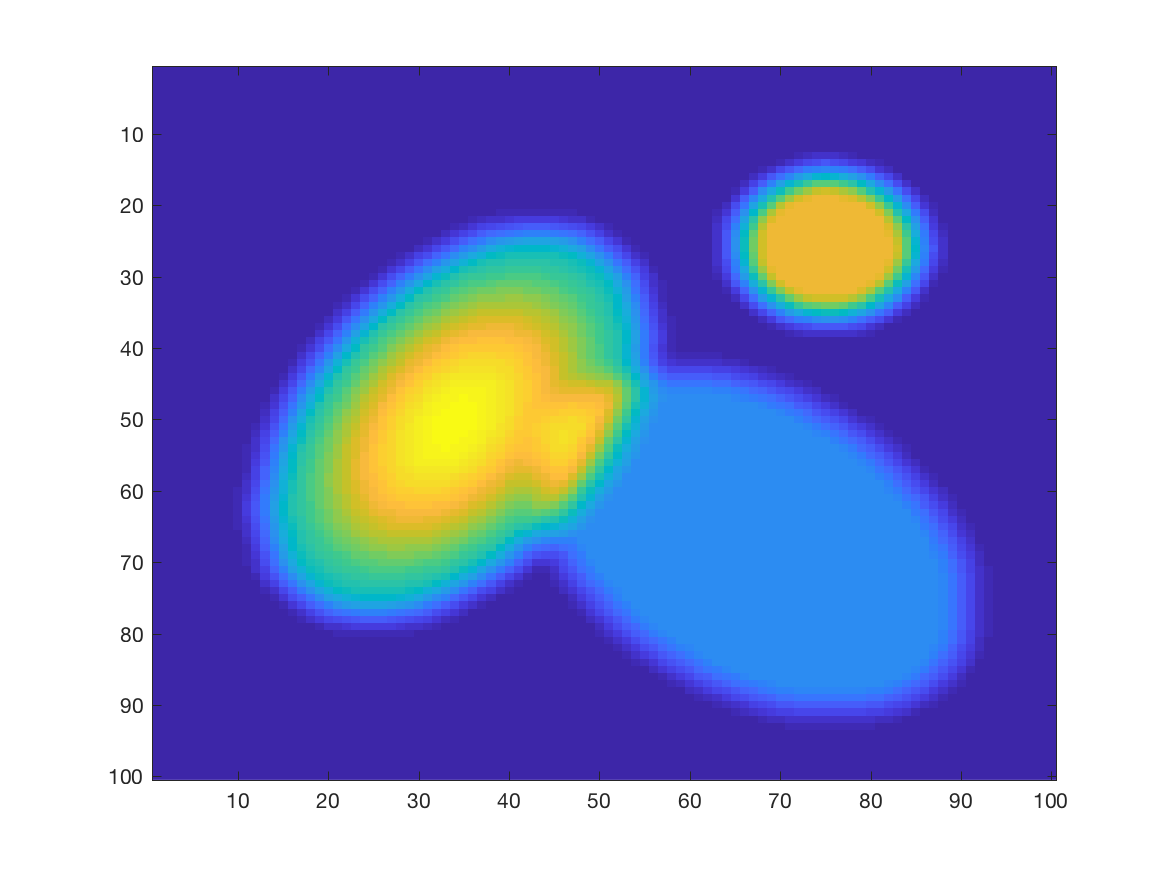
\includegraphics[width = 6.5cm]{blurredTarget.png} 
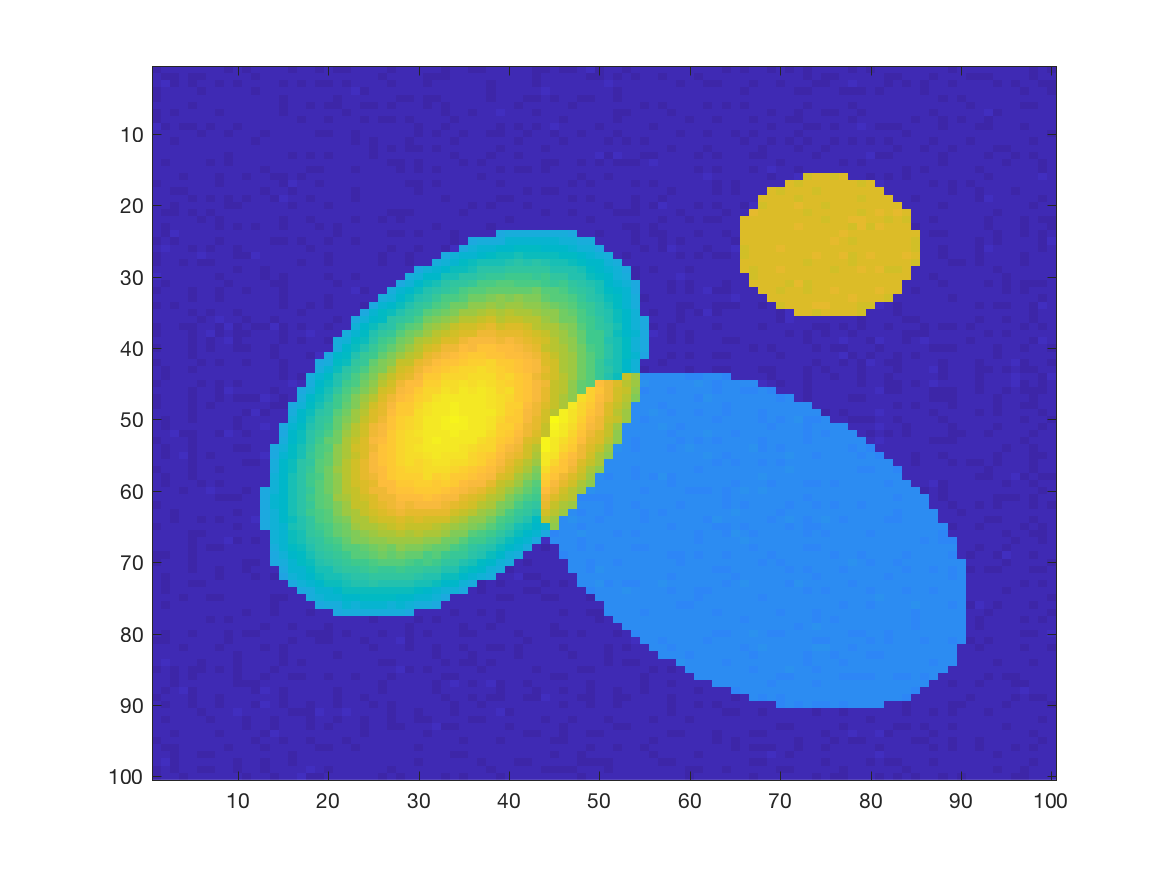
\includegraphics[width = 6.5cm]{TikhinovReconstructed.png} 
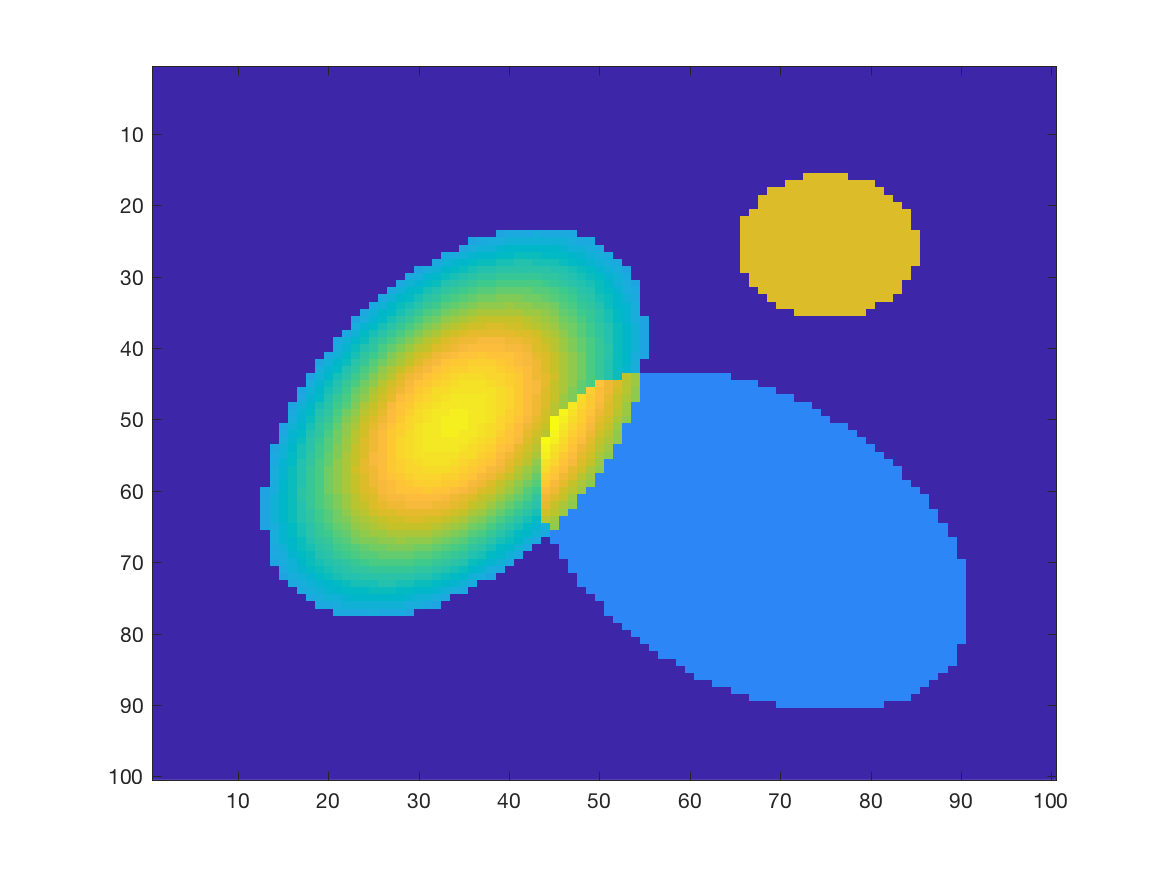
\includegraphics[width = 6.5cm]{TrueTarget.png}
}
\caption{\label{fig:Figure 6} The first panel shows the blurred image we used to set up the inverse problem, the second shows the reconstructed image using Tikhonov Regularization and the third shows the target image.}
\end{figure}

And finally, the code for finding this optimal alpha is given:

\begin{verbatim}
%% Reconstruction Further
tau = 1.2; % For tikhonov function, generally chosen as 
alphamin = 1e-16;
alphamax = 1e16;
discr0 = tau*norm(noise)^2;
delta = 0.001;
ddiscr = Inf;
iter = 0;
MAXITER = 10;
rnoise = sparse([bnoise;zeros(N,1)]);
solns = zeros(N,MAXITER); % stores the actual solutions in matrix column form
ddiscrs = zeros(1,MAXITER); % stores discrepancies
alphas = zeros(1,MAXITER); % stores the successive alphas
while (ddiscr > delta && iter < MAXITER)
    % Compute a regularized solution using the geometric mean
    iter = iter + 1;
    tic
    alpha = sqrt(alphamin*alphamax);
    alphas(iter) = alpha;
    x_alpha = (A'*A + alpha*eye(N))\(A'*bnoise);
    discr = norm(bnoise - A*x_alpha);
    toc
    % Geometric Bisection part.
    if discr > discr0
        alphamax = alpha;
    elseif discr <= discr0
        alphamin = alpha;
    end
    ddiscr = abs(discr - discr0);
    ddiscrs(iter) = ddiscr;
    solns(:,iter) = x_alpha;
end
\end{verbatim}

\end{document}